\documentclass[conference]{IEEEtran}
\IEEEoverridecommandlockouts
\usepackage{cite}
\usepackage{amsmath,amssymb,amsfonts}
\usepackage{graphicx}
\usepackage{booktabs}
\usepackage{textcomp}
\usepackage{xcolor}
\usepackage{url}
\usepackage{multirow}
% Native Bengali script requires XeLaTeX: fontspec + a Bengali-capable font.
% Compile with xelatex, not pdflatex (on Overleaf: Menu -> Compiler -> XeLaTeX).
% Font fallbacks: Windows has 'Times New Roman'/'Nirmala UI'; Overleaf (Linux)
% has 'TeX Gyre Termes' (Times clone) and the Noto Bengali fonts instead.
\usepackage{fontspec}
\IfFontExistsTF{Times New Roman}
  {\setmainfont{Times New Roman}[NFSSFamily=ptm]}
  {\setmainfont{TeX Gyre Termes}[NFSSFamily=ptm]}
\IfFontExistsTF{Nirmala UI}
  {\newfontfamily\bengalifont[Script=Bengali]{Nirmala UI}}
  {\IfFontExistsTF{Noto Serif Bengali}
    {\newfontfamily\bengalifont[Script=Bengali]{Noto Serif Bengali}}
    {\newfontfamily\bengalifont[Script=Bengali]{Noto Sans Bengali}}}
\newcommand{\bn}[1]{{\bengalifont #1}}
\def\BibTeX{{\rm B\kern-.05em{\sc i\kern-.025em b}\kern-.08em
    T\kern-.1667em\lower.7ex\hbox{E}\kern-.125emX}}
\begin{document}
% Standard camera-ready nudge: reclaim the last ~1cm of vertical space
% (a common, visually-unnoticeable adjustment used to fit page limits).
\addtolength{\textheight}{1.1cm}
\renewcommand{\arraystretch}{0.72}
% Standard camera-ready space trims: tighten the whitespace IEEEtran puts
% around floats/captions. Pure layout, no content is affected.
\setlength{\textfloatsep}{6pt plus 2pt minus 2pt}
\setlength{\floatsep}{4pt plus 2pt minus 2pt}
\setlength{\intextsep}{6pt plus 2pt minus 2pt}
\setlength{\abovecaptionskip}{3pt}
\setlength{\belowcaptionskip}{2pt}

\title{Bangla Word Sense Disambiguation: A Large-Scale Benchmark of Embedding and Classifier Combinations
}

\author{\IEEEauthorblockN{Prova Rani Paul}
\IEEEauthorblockA{\textit{Dept. of Computer Science and Engineering} \\
\textit{Khulna University of Engineering \& Technology}\\
Khulna, Bangladesh \\
provapaul123@gmail.com}
\and
\IEEEauthorblockN{Dr. K. M. Azharul Hasan}
\IEEEauthorblockA{\textit{Dept. of Computer Science and Engineering} \\
\textit{Khulna University of Engineering \& Technology}\\
Khulna, Bangladesh \\
az@cse.kuet.ac.bd}
}

\maketitle

\begin{abstract}
Word Sense Disambiguation for Bangla has so far relied on private datasets and hand-engineered features, and no prior study has fine-tuned a language model for the task. This paper presents a human-annotated Bangla WSD corpus of 12,059 sentences covering 402 ambiguous target words and 1,085 distinct sense glosses, with every sentence checked by two annotators on a web annotation platform built for this work; Cohen's kappa came out to 0.836 and 0.874 for the two annotators. We also run a controlled benchmark of 29 experiments on one fixed train/validation/test split: six text representations paired with three classical classifiers, four recurrent architectures over the two static embedding sequences, and three transformer backbones fine-tuned end to end. Word-specific labels remove cross-word sense collisions, leaving 1,048 sense classes over 373 words after filtering out rare senses. Fine-tuned BanglaBERT performs best, at 89.72\% test accuracy and 88.97\% weighted F1, while frozen BanglaBERT embeddings with logistic regression reach 89.30\% at roughly 70 times lower training cost. Under a target-word-constrained evaluation, lexical baselines improve by up to 58 accuracy points once predictions are restricted to the target word's own senses, but the strongest models barely move, meaning their remaining errors are confusions among senses of the same word rather than mistaken word identity. Together, these results establish transformer-based reference figures for Bangla Word Sense Disambiguation at this scale.
\end{abstract}

\begin{IEEEkeywords}
Word Sense Disambiguation, Bangla natural language processing, BanglaBERT, transformer tuning, low resource languages, sense-annotated corpus
\end{IEEEkeywords}

\section{Introduction}
Word Sense Disambiguation (WSD) is the task of choosing the correct sense of an ambiguous word from a predefined inventory, given its context \cite{ide1998wsd,navigli2009wsd}. It underlies machine translation, information retrieval, and question answering, where one mistranslated or misindexed polysemous word can invert a sentence's meaning. Bangla (Bengali), spoken by roughly 300 million people, is rich in exactly this kind of ambiguity: the word \bn{জল} (\emph{jal}) can mean water, rain, tears, or, idiomatically, exhausting toil, and only context tells these readings apart.

Yet Bangla WSD research has stayed confined to small, private datasets built on hand-engineered features. The five studies we found \cite{nazah2017,kaysarkhan2018,sahamoumittra2019,palsaha2019,dasdawn2023} evaluate on 160--3,860 sentences; none uses a learned embedding, none fine-tunes a transformer, only one dataset is public, and none reports inter-annotator reliability. Accuracies cluster between 77.5\% and 80.82\%, suggesting hand-engineered features have hit a ceiling that representation learning has never been asked to test.

This paper makes two contributions toward closing that gap: a new, large, sense-annotated Bangla WSD corpus, and a controlled 29-experiment benchmark built on it. The corpus holds 12,059 sentences covering 402 ambiguous target words and 1,085 sense glosses. The first 100 words were adopted from Das Dawn \emph{et al.}'s public dataset \cite{dasdawn2023}, and the remaining 302 words, along with every sentence and annotation, were newly contributed. It is, to our knowledge, the largest Bangla WSD corpus reported to date and the only one with quantified reliability (per-annotator Cohen's kappa of 0.836 and 0.874, ``almost perfect'' on the Landis--Koch scale \cite{cohen1960kappa,landis1977kappa}); a word-specific label scheme removes cross-word sense collisions, leaving 1,048 classes over 373 words after rare-sense filtering. The benchmark shares one fixed stratified 70/15/15 split (seed 42), one pipeline, and one evaluation suite across TF-IDF, pretrained Word2Vec \cite{mikolov2013word2vec} and fastText \cite{bojanowski2017fasttext}, frozen mBERT \cite{devlin2019bert}, BanglaBERT \cite{bhattacharjee2022banglabert}, and XLM-RoBERTa \cite{conneau2020xlmr}, four recurrent architectures, and end-to-end fine-tuning of all three transformers, scored both globally and under \emph{target-word-constrained} inference (restricting predictions to the target word's own senses, the realistic deployment setting). Fine-tuned BanglaBERT wins overall at 89.72\% accuracy and 88.97\% weighted F1, ahead of fine-tuned XLM-R by 3.7 points, mBERT by 5.6, and the best lexical baseline by more than 23. Frozen BanglaBERT with logistic regression lands within 0.42 points at a fraction of the cost; the constrained comparison shows the strongest models' remaining errors are almost entirely within-word. Section~II surveys related work, Section~III the corpus, Section~IV the benchmark methodology, Section~V results, and Section~VI concludes.

\section{Related Work}
\subsection{Word Sense Disambiguation}
WSD methodology has progressed through three generations \cite{navigli2009wsd}: knowledge-based methods matching context against dictionary glosses or WordNets, supervised classifiers over hand-engineered features, and representation learning built on distributed embeddings \cite{mikolov2013word2vec,bojanowski2017fasttext} and, most recently, pretrained transformers \cite{devlin2019bert}. Like all prior Bangla studies, this work adopts the lexical-sample (target-word) formulation, since no adequately covered all-words Bangla sense inventory yet exists.

\subsection{Bangla WSD}
Nazah \emph{et al.} \cite{nazah2017} pair Naive Bayes co-occurrence with a regression neural network for 77.5\% on 160 sentences over 50 words; Kaysar and Khan \cite{kaysarkhan2018} mine WSD as Apriori rules over co-occurrence vectors, reporting pattern-match counts rather than accuracy; Saha \emph{et al.} \cite{sahamoumittra2019} pair Levenshtein distance with cosine similarity for 80.82\% on 3,860 sentences over 100 words, the strongest classical result reviewed; Pal and Saha \cite{palsaha2019} apply unsupervised maximum-entropy clustering to 2,478 sentences over 7 words, improving 35\%$\to$61\% with PCA and WordNet expansion; and Das Dawn \emph{et al.} \cite{dasdawn2023} release the only public Bangla WSD dataset (100 words, 345 documents), reaching roughly 80\% with Random Forest under 10-fold cross-validation; their word list seeds the first 100 target words used here (Section~III). Across all five, none uses a learned embedding, none fine-tunes a transformer, only one dataset is public, and none reports inter-annotator agreement; this work addresses all three gaps.

\section{The Bangla WSD Corpus}
\subsection{Collection and Annotation}
The target-word inventory was built in two stages. The first 100 ambiguous words were adopted from the publicly available Bengali WSD dataset of Das Dawn \emph{et al.} \cite{dasdawn2023}\footnote{\url{https://www.kaggle.com/datasets/debapratimdasdawn/bengali-wsd-dataset}}, which we gratefully acknowledge as the starting point of this corpus; the remaining 302 ambiguous words were newly compiled for this work. For all 402 words, senses were validated against the \emph{Sansad Bangla Abhidhan} dictionary, and example sentences were gathered for each word--sense pair. Two annotators then checked every sentence independently on a PHP/MySQL annotation platform built for this work. The platform deduplicates imported sentences by SHA-256 hash, highlights the target word, shows the candidate senses in randomized order to reduce positional bias, and enforces through a database constraint that an annotator labels a given sentence only once.

Annotation reliability is quantified with Cohen's kappa \cite{cohen1960kappa}, computed per annotator against the platform's gold senses:
\begin{equation}
\kappa = \frac{p_o - p_e}{1 - p_e},
\label{eq:kappa}
\end{equation}
where $p_o$ is observed agreement and $p_e$ the agreement expected by chance from the marginal sense distributions. The two annotators obtained $\kappa = 0.836$ and $\kappa = 0.874$ (Fig.~\ref{fig:kappa}), both ``almost perfect'' on the Landis--Koch scale \cite{landis1977kappa}. No previous Bangla WSD dataset reports any reliability statistic.

\begin{figure}[!htbp]
\centerline{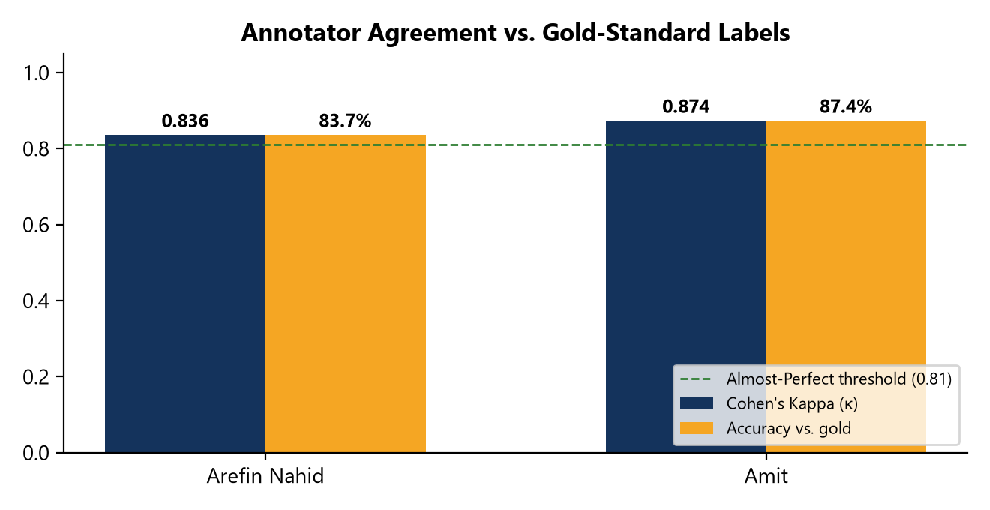
\includegraphics[width=0.44\columnwidth]{figs/kappa_agreement_chart.pdf}}
\caption{Per-annotator Cohen's kappa and raw accuracy against the gold senses; the dashed line is the 0.81 ``almost perfect'' threshold \cite{landis1977kappa}.}
\label{fig:kappa}
\end{figure}

Each corpus row records five fields: \texttt{word\_id}, \texttt{target\_word}, \texttt{sense\_id}, \texttt{sense\_gloss}, and \texttt{text}. Table~\ref{tab:sample} shows a snapshot of the \bn{রূপ} (\emph{rup}) block of the dataset: the target word stays the same while the sense moves from \bn{আকৃতি} (shape) through \bn{সৌন্দর্য} (beauty) to \bn{অবস্থা} (state), and only sentential context separates the readings.

\begin{table*}[tbp]
\caption{Snapshot of the proposed Bangla WSD dataset.}
\label{tab:sample}
\centering
\footnotesize
\setlength{\tabcolsep}{6pt}
\begin{tabular}{@{}cccll@{}}
\toprule
\texttt{word\_id} & \texttt{target\_word} & \texttt{sense\_id} & \texttt{sense\_gloss} & \texttt{text} \\
\midrule
114 & \bn{রূপ} & 1 & \bn{আকৃতি} & \bn{মেঘের রূপ ক্রমশ বদলে গিয়ে ঝড়ের আভাস দিচ্ছিল।} \\
114 & \bn{রূপ} & 1 & \bn{আকৃতি} & \bn{মোম গলে নতুন রূপ ধারণ করল।} \\
114 & \bn{রূপ} & 2 & \bn{সৌন্দর্য} & \bn{তার রূপ দেখে কবিরা অনেক কবিতা লিখেছেন।} \\
114 & \bn{রূপ} & 2 & \bn{সৌন্দর্য} & \bn{মা মেয়ের রূপ দেখে গর্বিত হলেন।} \\
114 & \bn{রূপ} & 3 & \bn{অবস্থা} & \bn{দেশের বর্তমান রূপ দেখে অনেকেই হতাশ।} \\
114 & \bn{রূপ} & 3 & \bn{অবস্থা} & \bn{যুদ্ধের পর শহরটির রূপ সম্পূর্ণ বদলে গেছে।} \\
$\vdots$ & $\vdots$ & $\vdots$ & $\vdots$ & $\vdots$ \\
\bottomrule
\end{tabular}
\end{table*}

\subsection{Preprocessing and Label Construction}
The raw corpus contains 12,059 sentences covering 402 unique target words and 1,085 distinct sense glosses. Fig.~\ref{fig:datasetstats} summarizes its composition: each word entry carries two to four candidate senses (202 entries with two, 75 with three, and 144 with four), nearly every word--sense class holds exactly ten sentences, and sentence lengths concentrate in the six-to-ten-word range (mean 8.8 words). Preprocessing normalizes whitespace, removes 874 rows whose target word does not appear verbatim in the sentence, and drops one exact duplicate, leaving 11,184 rows.

\begin{figure*}[!t]
\centerline{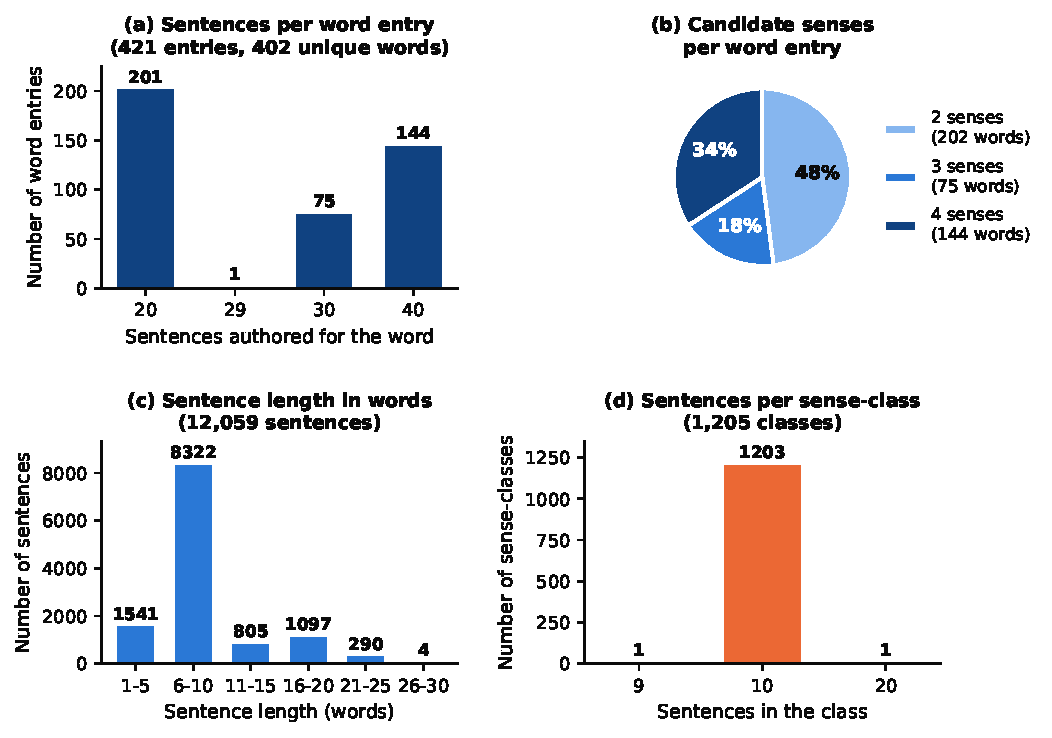
\includegraphics[width=0.64\textwidth]{figs/dataset_stats_overview.pdf}}
\caption{Composition of the raw corpus: (a) sentences authored per word entry, (b) candidate senses per word entry, (c) sentence-length distribution, and (d) sentences per word--sense class. Twenty target words are entered twice with separate sense inventories, giving 421 word entries over the 402 unique target words.}
\label{fig:datasetstats}
\end{figure*}

A naive use of raw sense identifiers would collide across words (sense 1 of one word sharing a label with sense 1 of another). We therefore construct \emph{word-specific labels} by concatenating the target word with its sense gloss, so every class is a unique (word, sense) pair. Classes with fewer than three examples are removed (33 rows). The final benchmark corpus holds \textbf{11,151 sentences, 373 target words, and 1,048 word--sense classes}, with 3--30 examples per class (mean 10.6) and a mean sentence length of 9.3 tokens. Table~\ref{tab:dataset} compares this corpus with all previously reported Bangla WSD datasets, and Table~\ref{tab:words} lists the complete target-word inventory with each word's number of candidate senses.

\begin{table}[tbp]
\caption{Comparison of existing Bangla WSD datasets with the proposed corpus.}
\label{tab:dataset}
\centering
\setlength{\tabcolsep}{4pt}
\begin{tabular}{@{}lllc@{}}
\toprule
\textbf{Source} & \textbf{Words} & \textbf{Sentences/Docs} & \textbf{Reliability} \\
\midrule
Pal and Saha \cite{palsaha2019} & 7 & 2,478 sent. & --- \\
Nazah \emph{et al.} \cite{nazah2017} & 50 & 160 sent. & --- \\
Saha \emph{et al.} \cite{sahamoumittra2019} & 100 & 3,860 sent. & --- \\
Kaysar and Khan \cite{kaysarkhan2018} & unspec. & 100--1,600 patt. & --- \\
Das Dawn \emph{et al.} \cite{dasdawn2023} & 100 & 345 docs & --- \\
\textbf{This work} & \textbf{402} & \textbf{12,059 sent.} & $\kappa$ = 0.836/0.874 \\
\bottomrule
\end{tabular}
\end{table}

\begin{table*}[!t]
\caption{Complete list of ambiguous target words in the proposed dataset, each with its number of candidate senses.}
\label{tab:words}
\centering
\scriptsize
\setlength{\tabcolsep}{1.6pt}
\begin{tabular}{@{}*{13}{c}@{}}
\toprule
\bn{অঙ্গ}~(4) & \bn{অজ}~(3) & \bn{অন্তর}~(3) & \bn{অন্ধকার}~(2) & \bn{অর্থ}~(3) & \bn{আঁচ}~(2) & \bn{আঁচল}~(2) & \bn{আকা}~(3) & \bn{আকাশ}~(2) & \bn{আগ}~(3) & \bn{আগুন}~(2) & \bn{আঙুল}~(2) & \bn{আটাশে}~(3) \\
\bn{আধার}~(4) & \bn{আয়না}~(2) & \bn{আলো}~(4) & \bn{আলোচ্য}~(4) & \bn{আসর}~(3) & \bn{আসা}~(2) & \bn{উঁচু}~(2) & \bn{উৎস}~(4) & \bn{এঁটে}~(2) & \bn{ওঠা}~(3) & \bn{কক্ষ}~(4) & \bn{কচ্ছপ}~(2) & \bn{কটা}~(3) \\
\bn{কড়া}~(3) & \bn{কড়ি}~(2) & \bn{কণা}~(4) & \bn{কণিকা}~(4) & \bn{কণ্ঠ}~(4) & \bn{কথা}~(3) & \bn{কপাল}~(2) & \bn{কপি}~(3) & \bn{কর}~(3) & \bn{করা}~(2) & \bn{কর্ণ}~(4) & \bn{কর্ম}~(2) & \bn{কল}~(4) \\
\bn{কলম}~(2) & \bn{কলা}~(2) & \bn{কলি}~(4) & \bn{কলিজা}~(2) & \bn{কাঁচা}~(2) & \bn{কাঁটা}~(2) & \bn{কাঁদা}~(2) & \bn{কাঁধ}~(2) & \bn{কাজ}~(2) & \bn{কাটা}~(3) & \bn{কাঠি}~(2) & \bn{কান}~(4) & \bn{কানা}~(3) \\
\bn{কাপ}~(3) & \bn{কাল}~(4) & \bn{কালা}~(4) & \bn{কালি}~(2) & \bn{কিরণ}~(4) & \bn{কুঁজো}~(3) & \bn{কুঠার}~(2) & \bn{কূল}~(4) & \bn{কেনা}~(2) & \bn{কেন্দ্র}~(4) & \bn{কোকিল}~(2) & \bn{কোল}~(2) & \bn{ক্ষেত্র}~(4) \\
\bn{খবর}~(2) & \bn{খাতা}~(2) & \bn{খারাপ}~(3) & \bn{খালি}~(2) & \bn{খুঁটি}~(2) & \bn{খুঁত}~(2) & \bn{খেলা}~(2) & \bn{খোলা}~(4) & \bn{গড়া}~(2) & \bn{গতি}~(4) & \bn{গভীর}~(3) & \bn{গরম}~(2) & \bn{গর্ভ}~(4) \\
\bn{গলা}~(3) & \bn{গা}~(3) & \bn{গাছ}~(2) & \bn{গাধা}~(2) & \bn{গান}~(2) & \bn{গাল}~(3) & \bn{গুণ}~(4) & \bn{গুল}~(3) & \bn{গোলা}~(4) & \bn{ঘটনা}~(2) & \bn{ঘড়ি}~(2) & \bn{ঘন}~(3) & \bn{ঘর}~(4) \\
\bn{ঘা}~(2) & \bn{ঘাট}~(3) & \bn{ঘাম}~(2) & \bn{ঘুম}~(2) & \bn{ঘোরা}~(2) & \bn{চক্র}~(4) & \bn{চটি}~(3) & \bn{চড়া}~(3) & \bn{চর}~(4) & \bn{চলা}~(3) & \bn{চাঁদ}~(2) & \bn{চাঁদা}~(4) & \bn{চাওয়া}~(2) \\
\bn{চাদর}~(2) & \bn{চাপ}~(2) & \bn{চাবি}~(4) & \bn{চামড়া}~(2) & \bn{চারা}~(2) & \bn{চাল}~(4) & \bn{চিনি}~(2) & \bn{চিল}~(2) & \bn{চিহ্ন}~(4) & \bn{চুন}~(2) & \bn{চূড়া}~(4) & \bn{চোখ}~(4) & \bn{ছত্র}~(3) \\
\bn{ছবক}~(2) & \bn{ছবি}~(2) & \bn{ছাঁচ}~(2) & \bn{ছাড়া}~(3) & \bn{ছাদ}~(2) & \bn{ছানি}~(2) & \bn{ছায়া}~(4) & \bn{ছুট}~(2) & \bn{ছোঁয়া}~(2) & \bn{জমি}~(3) & \bn{জল}~(3) & \bn{জাগা}~(2) & \bn{জানালা}~(2) \\
\bn{জাম}~(4) & \bn{জাল}~(3) & \bn{জিন}~(4) & \bn{জিভ}~(2) & \bn{জেতা}~(2) & \bn{জোয়ার}~(4) & \bn{জোর}~(2) & \bn{জ্বলা}~(2) & \bn{ঝড়}~(2) & \bn{ঝাঁক}~(2) & \bn{ঝাল}~(2) & \bn{ঝুড়ি}~(2) & \bn{ঝোলা}~(4) \\
\bn{টক}~(2) & \bn{টানা}~(3) & \bn{টিকা}~(4) & \bn{টিয়া}~(2) & \bn{টোকা}~(3) & \bn{ঠান্ডা}~(2) & \bn{ঠিক}~(3) & \bn{ডাক}~(4) & \bn{ডানা}~(2) & \bn{ডাল}~(4) & \bn{ঢালা}~(2) & \bn{ঢিবি}~(2) & \bn{তরঙ্গ}~(4) \\
\bn{তা}~(3) & \bn{তামা}~(2) & \bn{তার}~(3) & \bn{তারা}~(4) & \bn{তাল}~(4) & \bn{তালা}~(3) & \bn{তিল}~(2) & \bn{তীর}~(2) & \bn{তুফান}~(2) & \bn{তুলা}~(4) & \bn{তেজ}~(2) & \bn{তেতো}~(2) & \bn{তেল}~(2) \\
\bn{তোলা}~(2) & \bn{থাকা}~(2) & \bn{থোকা}~(2) & \bn{দণ্ড}~(4) & \bn{দম}~(4) & \bn{দরজা}~(2) & \bn{দল}~(3) & \bn{দাঁড়া}~(4) & \bn{দাঁড়ানো}~(2) & \bn{দাঁত}~(2) & \bn{দাগ}~(4) & \bn{দাম}~(2) & \bn{দিক}~(3) \\
\bn{দিন}~(2) & \bn{দিশা}~(4) & \bn{দুঃখ}~(2) & \bn{দুধ}~(2) & \bn{দৃষ্টি}~(4) & \bn{দেওয়া}~(2) & \bn{দেখা}~(3) & \bn{দোকান}~(2) & \bn{দ্বার}~(4) & \bn{ধন}~(4) & \bn{ধরা}~(4) & \bn{ধর্ম}~(2) & \bn{ধার}~(3) \\
\bn{ধারা}~(4) & \bn{নদী}~(4) & \bn{নয়}~(3) & \bn{নরম}~(2) & \bn{নাক}~(2) & \bn{নাম}~(2) & \bn{নামা}~(2) & \bn{নিঃশ্বাস}~(2) & \bn{নিচু}~(2) & \bn{নীল}~(3) & \bn{নুন}~(2) & \bn{নেওয়া}~(2) & \bn{নৌকা}~(2) \\
\bn{পড়া}~(3) & \bn{পথ}~(4) & \bn{পদ}~(4) & \bn{পর}~(3) & \bn{পর্দা}~(4) & \bn{পর্ব}~(4) & \bn{পা}~(4) & \bn{পাওয়া}~(2) & \bn{পাক}~(3) & \bn{পাকা}~(2) & \bn{পাকানো}~(4) & \bn{পাখা}~(2) & \bn{পাট}~(3) \\
\bn{পাতা}~(3) & \bn{পাত্র}~(4) & \bn{পাথর}~(4) & \bn{পান}~(4) & \bn{পানি}~(2) & \bn{পাল}~(4) & \bn{পালক}~(2) & \bn{পুষ্কর}~(4) & \bn{পৃষ্ঠা}~(4) & \bn{পেট}~(2) & \bn{পোকা}~(2) & \bn{প্রজাপতি}~(2) & \bn{প্রহর}~(4) \\
\bn{প্রান্ত}~(4) & \bn{ফল}~(4) & \bn{ফাঁক}~(2) & \bn{ফাঁকা}~(2) & \bn{ফাঁদ}~(2) & \bn{ফাটল}~(2) & \bn{ফিট}~(3) & \bn{ফুল}~(4) & \bn{বই}~(2) & \bn{বক}~(3) & \bn{বকা}~(2) & \bn{বকুল}~(2) & \bn{বড়ো}~(3) \\
\bn{বন্দর}~(4) & \bn{বন্ধ}~(2) & \bn{বর্ণ}~(3) & \bn{বর্তমান}~(3) & \bn{বল}~(4) & \bn{বসন্ত}~(2) & \bn{বসা}~(2) & \bn{বাঁক}~(2) & \bn{বাঁকা}~(2) & \bn{বাঁচা}~(2) & \bn{বাঁধ}~(4) & \bn{বাঁধা}~(2) & \bn{বাঁশি}~(2) \\
\bn{বাঘ}~(2) & \bn{বাচ্চা}~(2) & \bn{বাজার}~(2) & \bn{বাজি}~(4) & \bn{বাটা}~(3) & \bn{বাড়া}~(2) & \bn{বাড়ি}~(2) & \bn{বাতাস}~(2) & \bn{বাতি}~(2) & \bn{বাদাম}~(2) & \bn{বার}~(4) & \bn{বালি}~(2) & \bn{বাস}~(4) \\
\bn{বাহন}~(4) & \bn{বিছানা}~(2) & \bn{বিশ্বাস}~(2) & \bn{বিষ}~(2) & \bn{বিষয়}~(4) & \bn{বীজ}~(4) & \bn{বুক}~(4) & \bn{বৃত্ত}~(2) & \bn{বৃহস্পতি}~(4) & \bn{বেচা}~(2) & \bn{বেড়া}~(2) & \bn{বেল}~(4) & \bn{বেলা}~(3) \\
\bn{বোমা}~(3) & \bn{ব্যাঙ}~(2) & \bn{ভয়}~(2) & \bn{ভরা}~(2) & \bn{ভাগ্য}~(2) & \bn{ভাঙা}~(3) & \bn{ভাটা}~(4) & \bn{ভার}~(3) & \bn{ভারী}~(2) & \bn{ভালো}~(3) & \bn{ভাষা}~(4) & \bn{ভিজে}~(2) & \bn{ভিটা}~(2) \\
\bn{ভিত্তি}~(4) & \bn{মজা}~(3) & \bn{মঞ্চ}~(4) & \bn{মটকা}~(3) & \bn{মণি}~(4) & \bn{মধু}~(2) & \bn{ময়ূর}~(2) & \bn{মশাল}~(2) & \bn{মহল}~(3) & \bn{মহুরি}~(3) & \bn{মাটি}~(4) & \bn{মাঠ}~(2) & \bn{মাত}~(3) \\
\bn{মাত্রা}~(2) & \bn{মাথা}~(4) & \bn{মাধ্যম}~(4) & \bn{মান}~(4) & \bn{মাপকাঠি}~(4) & \bn{মায়া}~(2) & \bn{মারা}~(2) & \bn{মাল}~(4) & \bn{মিল}~(3) & \bn{মিষ্টি}~(2) & \bn{মুখ}~(4) & \bn{মুখোশ}~(4) & \bn{মুঠো}~(2) \\
\bn{মূল}~(4) & \bn{মেঘ}~(2) & \bn{মেরু}~(4) & \bn{মেলা}~(4) & \bn{মেশা}~(2) & \bn{মোটা}~(2) & \bn{মোড়}~(2) & \bn{মোম}~(2) & \bn{যাওয়া}~(2) & \bn{রং}~(2) & \bn{রক্ত}~(2) & \bn{রত্ন}~(4) & \bn{রথ}~(4) \\
\bn{রশ্মি}~(4) & \bn{রস}~(4) & \bn{রাখা}~(3) & \bn{রাগ}~(2) & \bn{রাজা}~(4) & \bn{রানী}~(4) & \bn{রাশি}~(4) & \bn{রাস্তা}~(2) & \bn{রূপ}~(4) & \bn{রেখা}~(4) & \bn{রোগ}~(2) & \bn{লজ্জা}~(2) & \bn{লম্বা}~(2) \\
\bn{লহরি}~(2) & \bn{লাই}~(4) & \bn{লাগা}~(3) & \bn{লেখা}~(2) & \bn{লেজ}~(2) & \bn{শক্ত}~(2) & \bn{শক্তি}~(4) & \bn{শাখা}~(4) & \bn{শানা}~(4) & \bn{শিকড়}~(2) & \bn{শিয়াল}~(2) & \bn{শিশু}~(3) & \bn{শোনা}~(2) \\
\bn{সংকেত}~(4) & \bn{সংসার}~(2) & \bn{সই}~(4) & \bn{সময়}~(4) & \bn{সমান}~(2) & \bn{সরা}~(3) & \bn{সরু}~(2) & \bn{সাজা}~(2) & \bn{সাদা}~(2) & \bn{সাপ}~(2) & \bn{সার}~(3) & \bn{সারা}~(3) & \bn{সিঁড়ি}~(2) \\
\bn{সিংহ}~(2) & \bn{সীমা}~(2) & \bn{সুর}~(4) & \bn{সূত্র}~(4) & \bn{সেতু}~(4) & \bn{সোজা}~(2) & \bn{স্তম্ভ}~(4) & \bn{স্পষ্ট}~(3) & \bn{স্বপ্ন}~(2) & \bn{স্বামী}~(2) & \bn{স্মৃতি}~(2) & \bn{হওয়া}~(2) & \bn{হল}~(3) \\
\bn{হাঁটা}~(2) & \bn{হাওয়া}~(2) & \bn{হাড়}~(2) & \bn{হাত}~(4) & \bn{হাতা}~(4) & \bn{হাতি}~(2) & \bn{হার}~(4) & \bn{হারানো}~(2) & \bn{হাসা}~(2) & \bn{হাসি}~(2) &  &  &  \\
\bottomrule
\end{tabular}
\end{table*}


\subsection{Target Marking and Data Split}
Each sentence is stored in two forms: marker-free for the lexical and static-embedding pipelines, and marked, with the target occurrence wrapped as \texttt{[TGT]} word \texttt{[/TGT]}, for the transformer pipelines. There the markers are registered as tokenizer special tokens with the embedding matrices resized to match, so they stay atomic instead of being split into subword pieces.

One fixed 70/15/15 train/validation/test split (seed 42) is created once and reused, with identical row indices, by every experiment. Because 18 of the 1,048 classes hold fewer than six examples, an exact three-way stratification is infeasible; we therefore stratify the train versus holdout division and split the holdout randomly into validation and test halves. The resulting sizes are 7,805 / 1,673 / 1,673 sentences, with all 1,048 classes present in training and 918 / 914 classes present in validation / test. All metrics are computed over the full label set with absent classes contributing zero, so no average is silently inflated. The test split is never used for model selection.

\section{Benchmark Methodology}
\subsection{Text Representations}
Six representations are generated under a shared fit-on-train, transform-all contract:

\subsubsection{TF-IDF} Word-level 1--2-grams, 30,000 maximum features, sublinear term frequency, fitted on the training split only.

\subsubsection{Pretrained static embeddings} Word2Vec and fastText are deliberately \emph{not} trained on the WSD corpus itself, which is far too small to learn reliable distributional vectors. Instead we load the pretrained 100-dimensional Bangla Word2Vec of \texttt{sagorsarker/bangla\_word2vec} (train-token coverage 98.0\%) and the official pretrained 300-dimensional Bengali fastText vectors (\texttt{wiki.bn}). The fastText subword $n$-grams produce usable vectors even for out-of-vocabulary inflected forms; coverage is 96.6\% from the known-word list alone. For the classical classifiers, both are formed into a \emph{target-aware} representation: the concatenation [left-context mean; target-word vector; right-context mean] with a five-word window on each side (300-D for Word2Vec, 900-D for fastText), rather than a whole-sentence mean that would dilute the disambiguation signal.

\subsubsection{Frozen transformer embeddings} mBERT (\texttt{bert-base-multilingual-cased}), BanglaBERT (\texttt{sagorsarker/bangla-bert-base}), and XLM-R (\texttt{xlm-roberta-base}) provide frozen contextual features: the concatenation of the \texttt{[CLS]} vector with the mean of the hidden states over the \texttt{[TGT]}-marked target span, giving 1,536 dimensions, with no gradient updates to the backbone.

\subsection{Classifier Grid and Sequence Models}
Three classical classifiers are trained on all six representations, giving 18 experiments: Gaussian/Multinomial Naive Bayes, logistic regression, and linear SVM, with features standardized on the training split for the latter two. Four recurrent architectures (LSTM, GRU, BiLSTM, BiGRU; hidden size 128, batch size 32, learning rate $10^{-3}$, up to 30 epochs with early-stopping patience 5) consume real per-token vector sequences padded/truncated to 20 tokens (the 95th percentile of training-sentence length). Sequence models are applied only to Word2Vec and fastText, the two representations with true token-level structure; feeding a recurrent network a single pooled vector is not sequence modeling, so those combinations are excluded. This yields 8 sequence experiments and $18 + 8 = 26$ grid experiments.

\subsection{Transformer Fine-Tuning}
The remaining three experiments fine-tune mBERT, BanglaBERT, and XLM-R end-to-end on the marked text. Each backbone's 768-D \texttt{[CLS]} representation feeds an identical classification head (LayerNorm, Dropout 0.3, Linear 768$\times$768, GELU, Dropout 0.3, Linear 768$\times$1048). Training uses AdamW (weight decay 0.01) with discriminative learning rates: the randomly initialized head receives ten times the backbone rate. The recipe also includes linear warm-up, class-balanced cross-entropy to counter the 1,048-class imbalance, gradient clipping at 1.0, bfloat16 mixed precision, batch size 16, maximum sequence length 128, and up to 15 epochs with early stopping. The checkpoint with the best validation accuracy is restored before the single final test evaluation. mBERT and BanglaBERT use a backbone rate of $2\times10^{-5}$ with 10\% warm-up; XLM-R collapsed under that recipe in preliminary runs and needed a gentler $1\times10^{-5}$ with 20\% warm-up. All runs used a Tesla T4 GPU (15.6 GB) with PyTorch.

\subsection{Evaluation Protocol}
Every experiment is scored on the held-out test split with accuracy, macro- and weighted-averaged precision/recall/F1, balanced accuracy, Matthews correlation coefficient (MCC), and Cohen's kappa (here as a model-agreement statistic). Macro averages weight all 1,048 classes equally and are pulled down by rare senses with one or two test examples; weighted averages reflect the actual test distribution. Both are reported.

In addition to this \emph{global} evaluation, every model is evaluated under \emph{target-word-constrained} inference. In realistic use, the target word $w_i$ of test sentence $i$ is known at prediction time and only its own candidate senses are legitimate answers. With $s_{ik}$ the model's native score for class $k$ on sentence $i$ and $\mathcal{L}(w_i)$ the set of label indices belonging to $w_i$, the constrained prediction restricts the arg-max to that subset:
\begin{equation}
\hat{y}_i^{\,\mathrm{c}} = \operatorname*{arg\,max}_{k \,\in\, \mathcal{L}(w_i)} \; s_{ik}.
\label{eq:constrained}
\end{equation}
This is an inference-time restriction only: the same trained model and score matrix are reused, and no per-word classifier is ever trained. The gap between global and constrained scores is diagnostic: a model whose errors are mostly cross-word gains greatly from the restriction, whereas a model whose errors already lie within the correct word's sense set gains almost nothing.

\section{Results and Discussion}
\subsection{Overall Benchmark}
Table~\ref{tab:main} reports the complete 29-experiment benchmark on the test split, and Fig.~\ref{fig:acc} visualizes the accuracy ranking. Three findings stand out.

\begin{table}[tbp]
\caption{Performance of all 29 embedding--classifier combinations on the held-out test split (1,673 sentences, global evaluation over all 1,048 classes). All values except MCC in \%.}
\label{tab:main}
\centering
\scriptsize
\setlength{\tabcolsep}{3.4pt}
\begin{tabular}{@{}llrrrr@{}}
\toprule
\textbf{Embedding} & \textbf{Model} & \textbf{Acc.} & \textbf{M-F1} & \textbf{W-F1} & \textbf{MCC} \\
\midrule
TF-IDF & Naive Bayes & 14.23 & 8.85 & 12.96 & 0.157 \\
TF-IDF & Log. Regression & 63.72 & 51.53 & 61.01 & 0.637 \\
TF-IDF & Linear SVM & 66.35 & 54.19 & 64.56 & 0.663 \\
\midrule
Word2Vec & Naive Bayes & 61.09 & 49.46 & 59.08 & 0.611 \\
Word2Vec & Log. Regression & 74.48 & 62.34 & 73.15 & 0.745 \\
Word2Vec & Linear SVM & 63.42 & 51.04 & 60.63 & 0.634 \\
Word2Vec & LSTM & 13.27 & 9.33 & 12.09 & 0.132 \\
Word2Vec & GRU & 29.05 & 20.53 & 26.65 & 0.290 \\
Word2Vec & BiLSTM & 58.46 & 46.12 & 55.67 & 0.584 \\
Word2Vec & BiGRU & 60.67 & 47.73 & 57.65 & 0.606 \\
\midrule
fastText & Naive Bayes & 61.92 & 50.36 & 59.84 & 0.619 \\
fastText & Log. Regression & 85.06 & 71.42 & 83.61 & 0.850 \\
fastText & Linear SVM & 79.74 & 66.30 & 78.26 & 0.797 \\
fastText & LSTM & 25.40 & 17.80 & 22.71 & 0.253 \\
fastText & GRU & 53.56 & 42.05 & 51.13 & 0.535 \\
fastText & BiLSTM & 70.23 & 57.35 & 68.05 & 0.702 \\
fastText & BiGRU & 71.49 & 58.67 & 69.47 & 0.715 \\
\midrule
mBERT (frozen) & Naive Bayes & 75.85 & 63.54 & 74.65 & 0.758 \\
mBERT (frozen) & Log. Regression & 79.74 & 67.42 & 78.37 & 0.797 \\
mBERT (frozen) & Linear SVM & 75.49 & 62.86 & 73.45 & 0.755 \\
\midrule
XLM-R (frozen) & Naive Bayes & 85.89 & 72.00 & 84.66 & 0.859 \\
XLM-R (frozen) & Log. Regression & 86.55 & 73.68 & 85.75 & 0.865 \\
XLM-R (frozen) & Linear SVM & 85.77 & 72.15 & 84.55 & 0.858 \\
\midrule
BanglaBERT (frozen) & Naive Bayes & 85.59 & 72.52 & 85.05 & 0.856 \\
BanglaBERT (frozen) & Log. Regression & 89.30 & 76.04 & 88.61 & 0.893 \\
BanglaBERT (frozen) & Linear SVM & 88.22 & 75.11 & 87.43 & 0.882 \\
\midrule
mBERT & Fine-tuned & 84.16 & 71.68 & 83.59 & 0.841 \\
XLM-R & Fine-tuned & 86.01 & 73.05 & 85.02 & 0.860 \\
BanglaBERT & \textbf{Fine-tuned} & \textbf{89.72} & \textbf{76.42} & \textbf{88.97} & \textbf{0.897} \\
\bottomrule
\end{tabular}
\end{table}

\begin{figure}[tbp]
\centerline{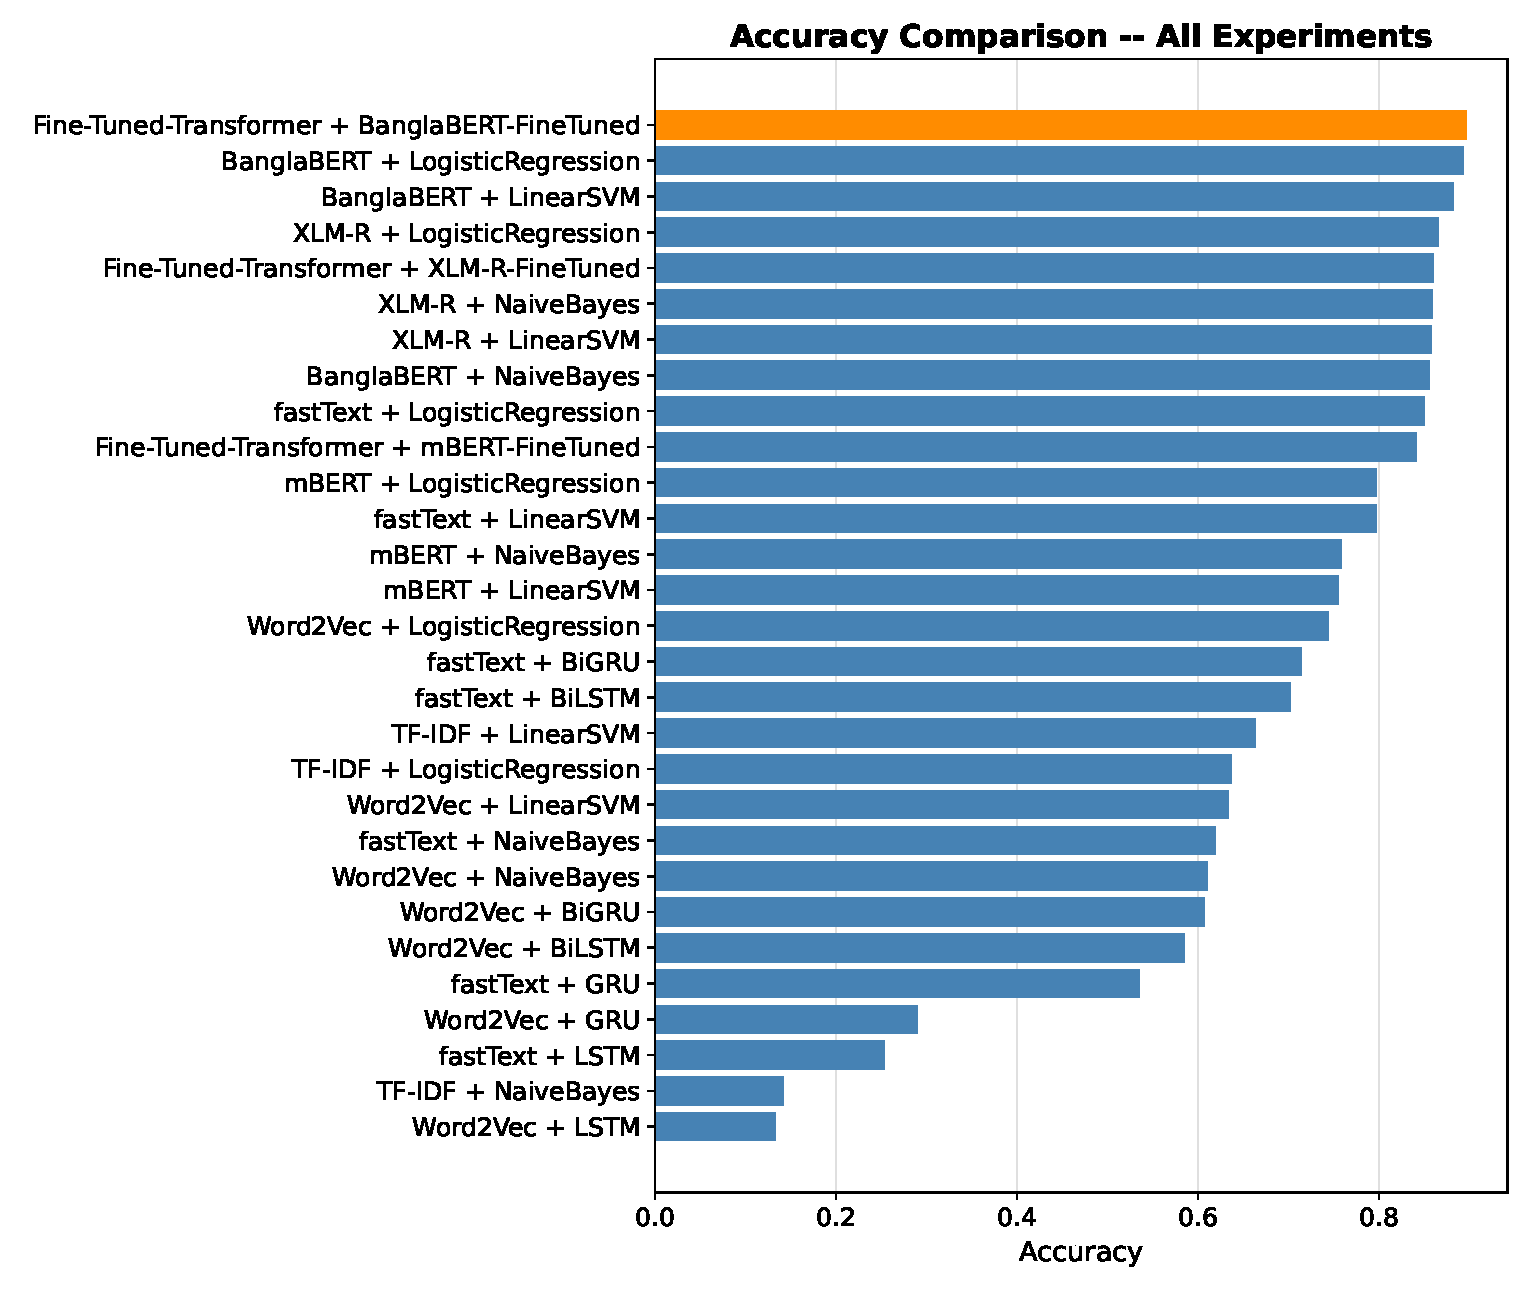
\includegraphics[width=0.5\columnwidth]{figs/comparison_accuracy.pdf}}
\caption{Test accuracy of all 29 embedding--classifier configurations under the global 1,048-class evaluation. Transformer-based representations dominate, with fine-tuned BanglaBERT best overall.}
\label{fig:acc}
\end{figure}

\textbf{Representation quality dominates.} Holding the classifier fixed at logistic regression, accuracy climbs monotonically with representation quality: 63.72\% (TF-IDF), 74.48\% (Word2Vec), 85.06\% (fastText), 79.74\% (frozen mBERT), 86.55\% (frozen XLM-R), and 89.30\% (frozen BanglaBERT). That 23-point spread between the best lexical and best contextual pipeline dwarfs any within-representation classifier difference, so Bangla WSD is bottlenecked by representation, not classifier choice. Subword-aware fastText outperforms word-level Word2Vec ($+10.6$ points with logistic regression), consistent with Bangla's heavy inflectional morphology.

\textbf{Language-specific pretraining beats multilingual scale.} Under identical conditions, BanglaBERT outperforms both multilingual backbones in every configuration: frozen, it beats frozen XLM-R by 2.8 and frozen mBERT by 9.6 accuracy points; fine-tuned, it beats fine-tuned XLM-R by 3.7 and fine-tuned mBERT by 5.6 points. Monolingual pretraining evidently buys more Bangla-relevant capacity than mBERT and XLM-R's hundredfold-larger multilingual corpora.

\textbf{Recurrent models underperform their classical counterparts.} Every RNN trails the logistic-regression model on the same embedding (best RNN: fastText BiGRU at 71.49\% vs. 85.06\% for fastText with logistic regression). At roughly 7.4 training sentences per class, sequence encoders overfit before exploiting word order, while target-aware pooled features hand the classical models exactly the signal that matters; unidirectional variants suffer most (Word2Vec LSTM: 13.27\%) since the disambiguating context often lies to the target word's right.

\subsection{Fine-Tuning versus Frozen Features}
Fine-tuned BanglaBERT is the best model overall (89.72\% accuracy, 88.97\% weighted F1, MCC 0.897), but its margin over frozen BanglaBERT features with logistic regression is only 0.42 points, and the cost asymmetry is stark: fine-tuning ran roughly 64 minutes on a T4 GPU, versus under a minute for embedding extraction plus logistic-regression training, a 70-fold difference. Frozen BanglaBERT with a linear head is thus a near-optimal substitute for deployments without a GPU training budget. Fig.~\ref{fig:curves} shows the fine-tuned BanglaBERT training trajectory; validation accuracy plateaus after roughly ten epochs, and early stopping prevents overfitting.

\begin{figure}[tbp]
\centerline{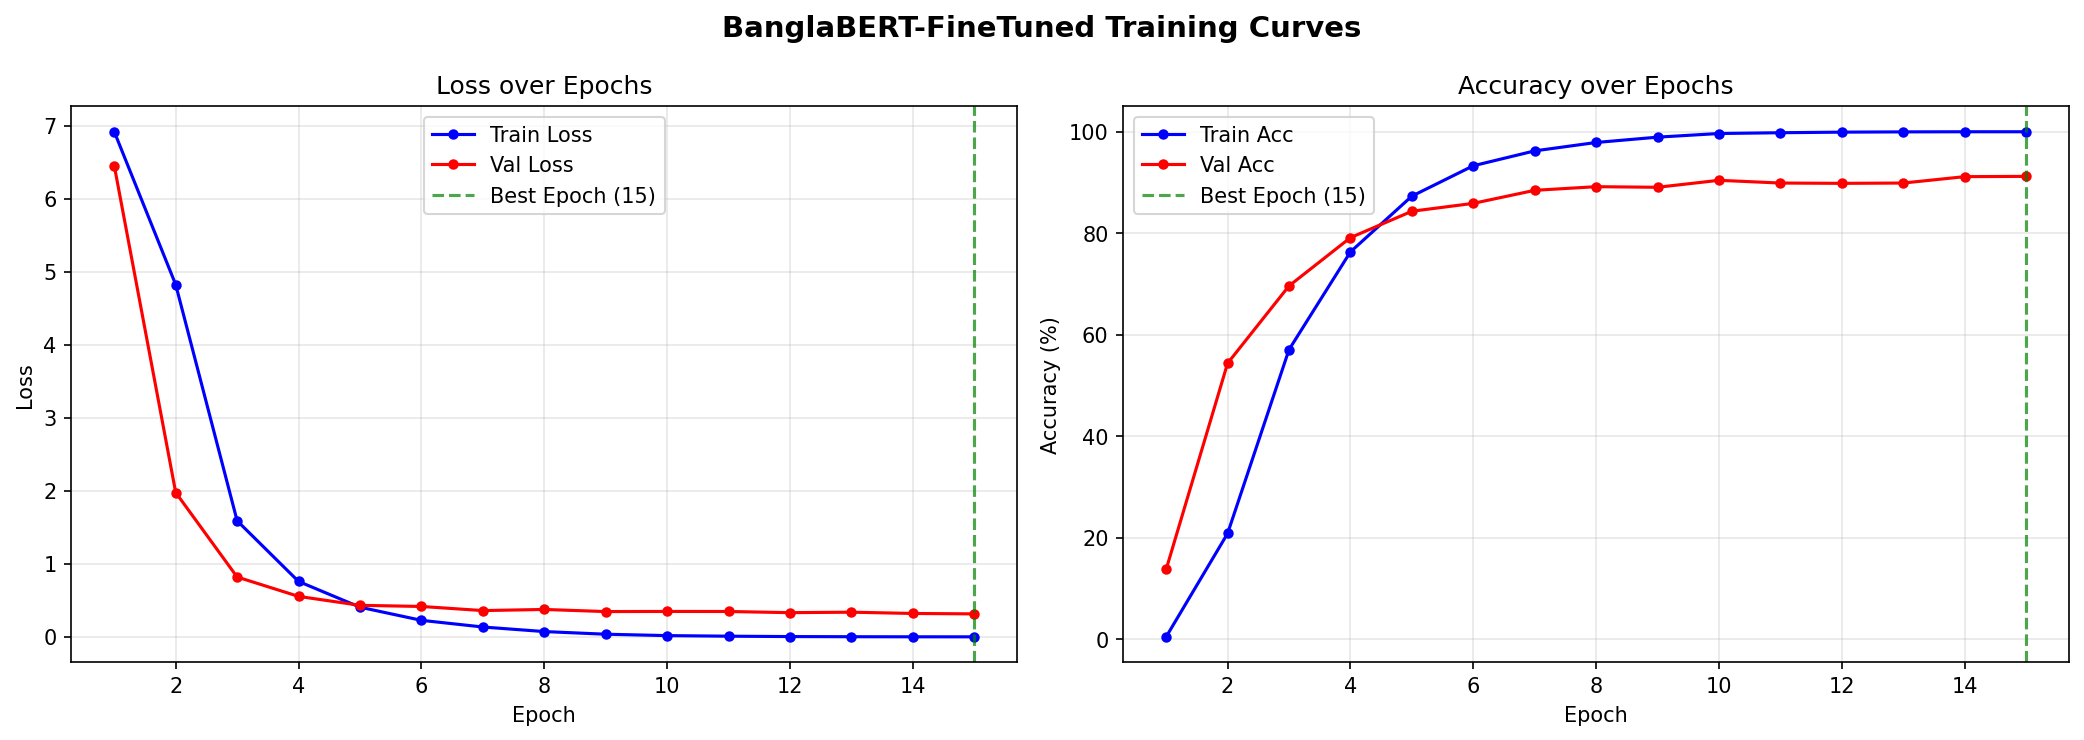
\includegraphics[width=0.95\columnwidth]{figs/BanglaBERT-FineTuned_training_curves.png}}
\caption{Training and validation loss/accuracy curves for fine-tuned BanglaBERT. The best-validation checkpoint is restored before the final test evaluation.}
\label{fig:curves}
\end{figure}

The XLM-R result carries a methodological caution. Under the learning-rate policy that trains mBERT and BanglaBERT without incident, XLM-R fine-tuning collapsed; only a halved backbone learning rate with doubled warm-up produced its 86.01\% result. Benchmark comparisons that fine-tune all backbones under one blind recipe risk reporting an optimization artifact as a model ranking.

\subsection{Global versus Target-Word-Constrained Evaluation}
Table~\ref{tab:constrained} contrasts global and constrained scores (\ref{eq:constrained}) for representative models, and Fig.~\ref{fig:constrained} plots the full picture. The restriction transforms weak models: TF-IDF Naive Bayes jumps from 14.23\% to 72.44\% ($+58.2$ points) and Word2Vec LSTM from 13.27\% to 62.94\%, since their global scores are dominated by \emph{cross-word} errors (predicting a sense of an entirely different word) that the constraint removes for free. The strongest models barely move: fine-tuned BanglaBERT gains 0.06 points (89.72\% to 89.78\%) and fine-tuned mBERT gains exactly zero, because their errors are almost entirely within-word sense confusions, which constrained inference cannot fix. Two practical conclusions follow: a deployed Bangla WSD system should always apply the cost-free constraint, and future gains for strong models must come from better sense discrimination, not better word identification.

\begin{table}[tbp]
\caption{Effect of target-word-constrained inference on test accuracy (\%) for representative models.}
\label{tab:constrained}
\centering
\scriptsize
\setlength{\tabcolsep}{4.5pt}
\begin{tabular}{@{}lrrr@{}}
\toprule
\textbf{Model} & \textbf{Global} & \textbf{Constrained} & \textbf{Gain} \\
\midrule
TF-IDF + Naive Bayes & 14.23 & 72.44 & $+58.21$ \\
Word2Vec + LSTM & 13.27 & 62.94 & $+49.67$ \\
Word2Vec + BiLSTM & 58.46 & 78.54 & $+20.08$ \\
TF-IDF + Linear SVM & 66.35 & 72.38 & $+6.03$ \\
Word2Vec + Log. Regr. & 74.48 & 80.10 & $+5.62$ \\
fastText + Log. Regr. & 85.06 & 85.30 & $+0.24$ \\
XLM-R (frozen) + Log. Regr. & 86.55 & 87.39 & $+0.84$ \\
BanglaBERT (frozen) + Log. Regr. & 89.30 & 89.54 & $+0.24$ \\
mBERT fine-tuned & 84.16 & 84.16 & $0.00$ \\
XLM-R fine-tuned & 86.01 & 86.07 & $+0.06$ \\
BanglaBERT fine-tuned & \textbf{89.72} & \textbf{89.78} & $+0.06$ \\
\bottomrule
\end{tabular}
\end{table}

\begin{figure}[tbp]
\centerline{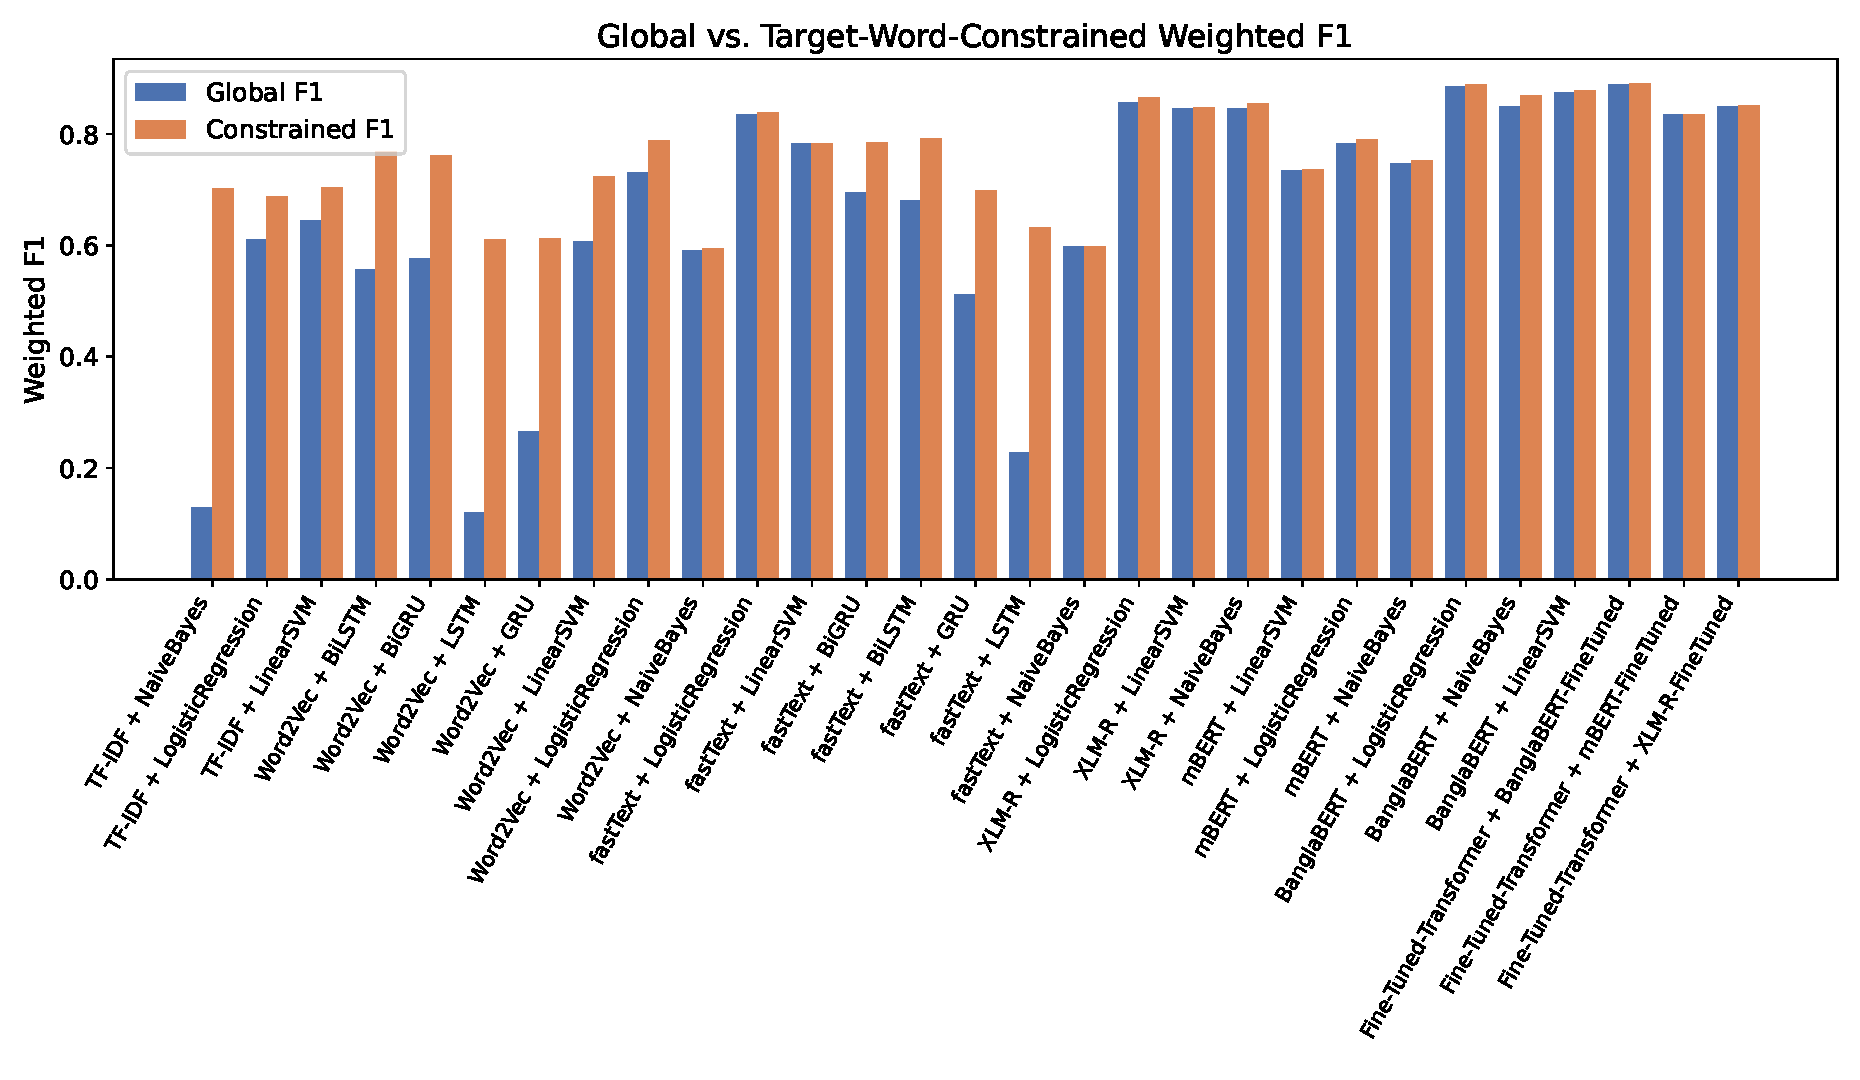
\includegraphics[width=0.95\columnwidth]{figs/global_vs_constrained_f1.pdf}}
\caption{Global versus target-word-constrained weighted F1 for all 29 configurations. Weak models close most of their gap under the constraint; strong models are nearly unchanged.}
\label{fig:constrained}
\end{figure}

\subsection{Comparison with Prior Bangla WSD Work}
Direct numeric comparison with prior studies is necessarily approximate, since each was evaluated on its own private dataset, but context still matters: the strongest previously reported Bangla WSD accuracy is 80.82\% on 100 target words \cite{sahamoumittra2019}, with other supervised studies reporting 77.5--80\% on 50--100 words \cite{nazah2017,dasdawn2023}. Fine-tuned BanglaBERT reaches 89.72\% on a harder task along every axis: 373 target words, a 1,048-class label space, and three to four times more sentences than the largest prior dataset. The benchmark also sets a useful negative reference point: hand-engineered TF-IDF with the standard Naive Bayes pairing common in the prior literature collapses to 14.23\% once the label space is realistic and collision-free.

\subsection{Limitations}
The corpus's sense inventory follows a single dictionary and averages 10.6 sentences per sense, so rare senses remain hard (macro F1 trails weighted F1 by roughly 12 points for all strong models). Validation and test splits omit some of the 1,048 classes (918 and 914 present, respectively) since 18 classes hold fewer than six examples; metrics are computed over the full label set so averages are not inflated, and results are single-run on one fixed split by design, resting on pattern consistency across all 29 experiments rather than repeated runs.

\section{Conclusion}
This paper introduced the largest reliability-checked Bangla WSD corpus to date (12,059 sentences, 402 ambiguous words, 1,085 sense glosses, kappa of 0.836 and 0.874) alongside the first controlled Bangla WSD benchmark spanning lexical features, static embeddings, recurrent models, and frozen and fine-tuned transformers: 29 experiments on one split, one pipeline, one metric suite. Fine-tuned BanglaBERT sets the reference figure at 89.72\% accuracy (88.97\% weighted F1) over 1,048 word--sense classes, ahead of mBERT and XLM-R under identical recipes and of every prior reported Bangla WSD accuracy on a far harder label space; frozen BanglaBERT features with logistic regression reach 89.30\% at roughly 70 times lower cost, and the constrained evaluation shows that what still limits the strong models is telling apart senses of the same word. Future work includes examples for rare senses, parameter-efficient fine-tuning, and moving toward all-words Bangla WSD as sense-inventory coverage improves.

\begin{thebibliography}{00}
\bibitem{ide1998wsd} N. Ide and J. V\'eronis, ``Word sense disambiguation: The state of the art,'' \textit{Computational Linguistics}, vol. 24, no. 1, pp. 1--40, 1998.
\bibitem{navigli2009wsd} R. Navigli, ``Word sense disambiguation: A survey,'' \textit{ACM Computing Surveys}, vol. 41, no. 2, pp. 1--69, 2009.
\bibitem{mikolov2013word2vec} T. Mikolov, K. Chen, G. Corrado, and J. Dean, ``Efficient estimation of word representations in vector space,'' arXiv:1301.3781, 2013.
\bibitem{bojanowski2017fasttext} P. Bojanowski, E. Grave, A. Joulin, and T. Mikolov, ``Enriching word vectors with subword information,'' \textit{Trans. Assoc. Comput. Linguistics}, vol. 5, pp. 135--146, 2017.
\bibitem{devlin2019bert} J. Devlin, M.-W. Chang, K. Lee, and K. Toutanova, ``BERT: Pre-training of deep bidirectional transformers for language understanding,'' in \textit{Proc. NAACL-HLT}, 2019, pp. 4171--4186.
\bibitem{conneau2020xlmr} A. Conneau \emph{et al.}, ``Unsupervised cross-lingual representation learning at scale,'' in \textit{Proc. ACL}, 2020, pp. 8440--8451.
\bibitem{bhattacharjee2022banglabert} A. Bhattacharjee \emph{et al.}, ``BanglaBERT: Language model pretraining and benchmarks for low-resource language understanding evaluation in Bangla,'' in \textit{Findings of NAACL}, 2022, pp. 1318--1327.
\bibitem{cohen1960kappa} J. Cohen, ``A coefficient of agreement for nominal scales,'' \textit{Educational and Psychological Measurement}, vol. 20, no. 1, pp. 37--46, 1960.
\bibitem{landis1977kappa} J. R. Landis and G. G. Koch, ``The measurement of observer agreement for categorical data,'' \textit{Biometrics}, vol. 33, no. 1, pp. 159--174, 1977.
\bibitem{nazah2017} S. Nazah, M. M. Hoque, and M. R. Hossain, ``Word sense disambiguation of Bangla sentences using statistical approach,'' in \textit{Proc. IEEE 3rd Int. Conf. Electrical Information and Communication Technology (EICT)}, 2017.
\bibitem{kaysarkhan2018} M. S. Kaysar and M. I. Khan, ``Word sense disambiguation for Bangla words using Apriori algorithm,'' in \textit{Proc. ICRAMPS}, 2018.
\bibitem{sahamoumittra2019} P. K. Saha, A. D. Mou, and T. Mittra, ``A Bangla word sense disambiguation technique using minimum edit distance algorithm and cosine distance,'' in \textit{Proc. IEEE}, 2019.
\bibitem{palsaha2019} A. R. Pal and D. Saha, ``Word sense disambiguation in Bengali language using unsupervised methodology with modifications,'' \textit{S\=adhan\=a}, vol. 44, no. 168, pp. 1--13, 2019.
\bibitem{dasdawn2023} D. Das Dawn, A. Khan, S. H. Shaikh, and R. K. Pal, ``A dataset for evaluating Bengali word sense disambiguation techniques,'' \textit{J. Ambient Intelligence and Humanized Computing}, vol. 14, pp. 4057--4086, 2023.
\end{thebibliography}

\end{document}
